\documentclass[12pt]{article}

%%%<
\usepackage{verbatim}
%\usepackage[active,tightpage]{preview}
%\PreviewEnvironment{tikzpicture}
%\setlength\PreviewBorder{5pt}%
%%%>
\usepackage[x11names]{xcolor}                     %Additional colors
\usepackage{euler}                                %Nicer numbers
\usepackage{tikz}
\usepackage{pgfplots}
\usepgfplotslibrary{polar}
\usetikzlibrary{calc, arrows, patterns,angles ,positioning,quotes}
\usetikzlibrary{decorations.markings}
\usetikzlibrary{arrows.meta}

%==== Chinese Setting  ====== 

\input{E:/NCTUG2/TEX/LatexCodeTemplate/inputFile/Qheader.tex}


\begin{document}

    \newcommand{\drawHDYXYaxes}{
        \draw[->] (-2.2,0) -- (2.2,0);
        \draw[->] (0,-2.2) -- (0,2.2);
        }
    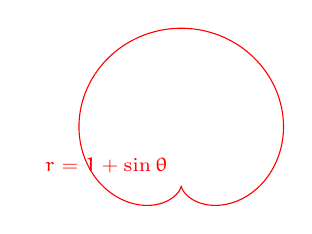
\begin{tikzpicture}[scale=1]
    \drawHDYXYaxes
    \draw node [red] at (-1,.25) {\scriptsize{ $r=1+\sin
            \theta$}};
    \draw[color=red,domain=0:6.28,samples=200,smooth] plot (canvas polar
    cs:angle=\x r,radius=      {1cm+1cm*sin(\x r)});    %r = angle en radian
    \end{tikzpicture}
    
    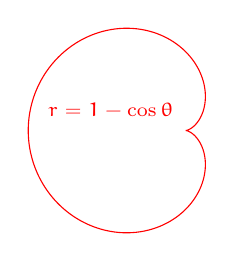
\begin{tikzpicture}[scale=1]
    \drawHDYXYaxes
    
    \draw node [red] at (-1,.25) {\scriptsize{ $r=1-\cos
            \theta$}};
    \draw[color=red,domain=0:6.28,samples=200,smooth] plot (canvas polar
    cs:angle=\x r,radius=      {1cm-1cm*cos(\x r)});    %r = angle en radian
    \end{tikzpicture}
    
    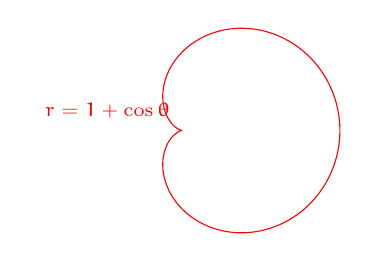
\begin{tikzpicture}[scale=1]
    \drawHDYXYaxes
    
    \draw node [red] at (-1,.25) {\scriptsize{ $r=1+\cos
            \theta$}};
    \draw[color=red,domain=0:6.28,samples=200,smooth] plot (canvas polar
    cs:angle=\x r,radius=      {1cm+1cm*cos(\x r)});    %r = angle en radian
    \end{tikzpicture}
    
    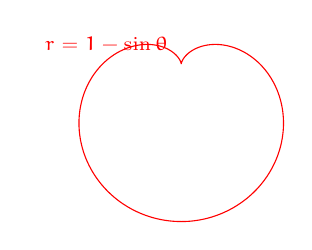
\begin{tikzpicture}[scale=1]
    \drawHDYXYaxes
    
    \draw node [red] at (-1,.25) {\scriptsize{ $r=1-\sin
            \theta$}};
    \draw[color=red,domain=0:6.28,samples=200,smooth] plot (canvas polar
    cs:angle=\x r,radius=      {1cm-1cm*sin(\x r)});    %r = angle en radian
    \end{tikzpicture}
    
        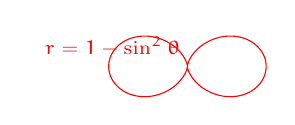
\begin{tikzpicture}[scale=1]
        \drawHDYXYaxes
        
        \draw node [red] at (-1,.25) {\scriptsize{ $r=1-\sin^2
                \theta$}};
        \draw[color=red,domain=0:6.28,samples=200,smooth] plot (canvas polar
        cs:angle=\x r,radius=      {1cm-1cm*sin(\x r)*sin(\x r)});    %r = angle en radian
        \end{tikzpicture}
        
    
    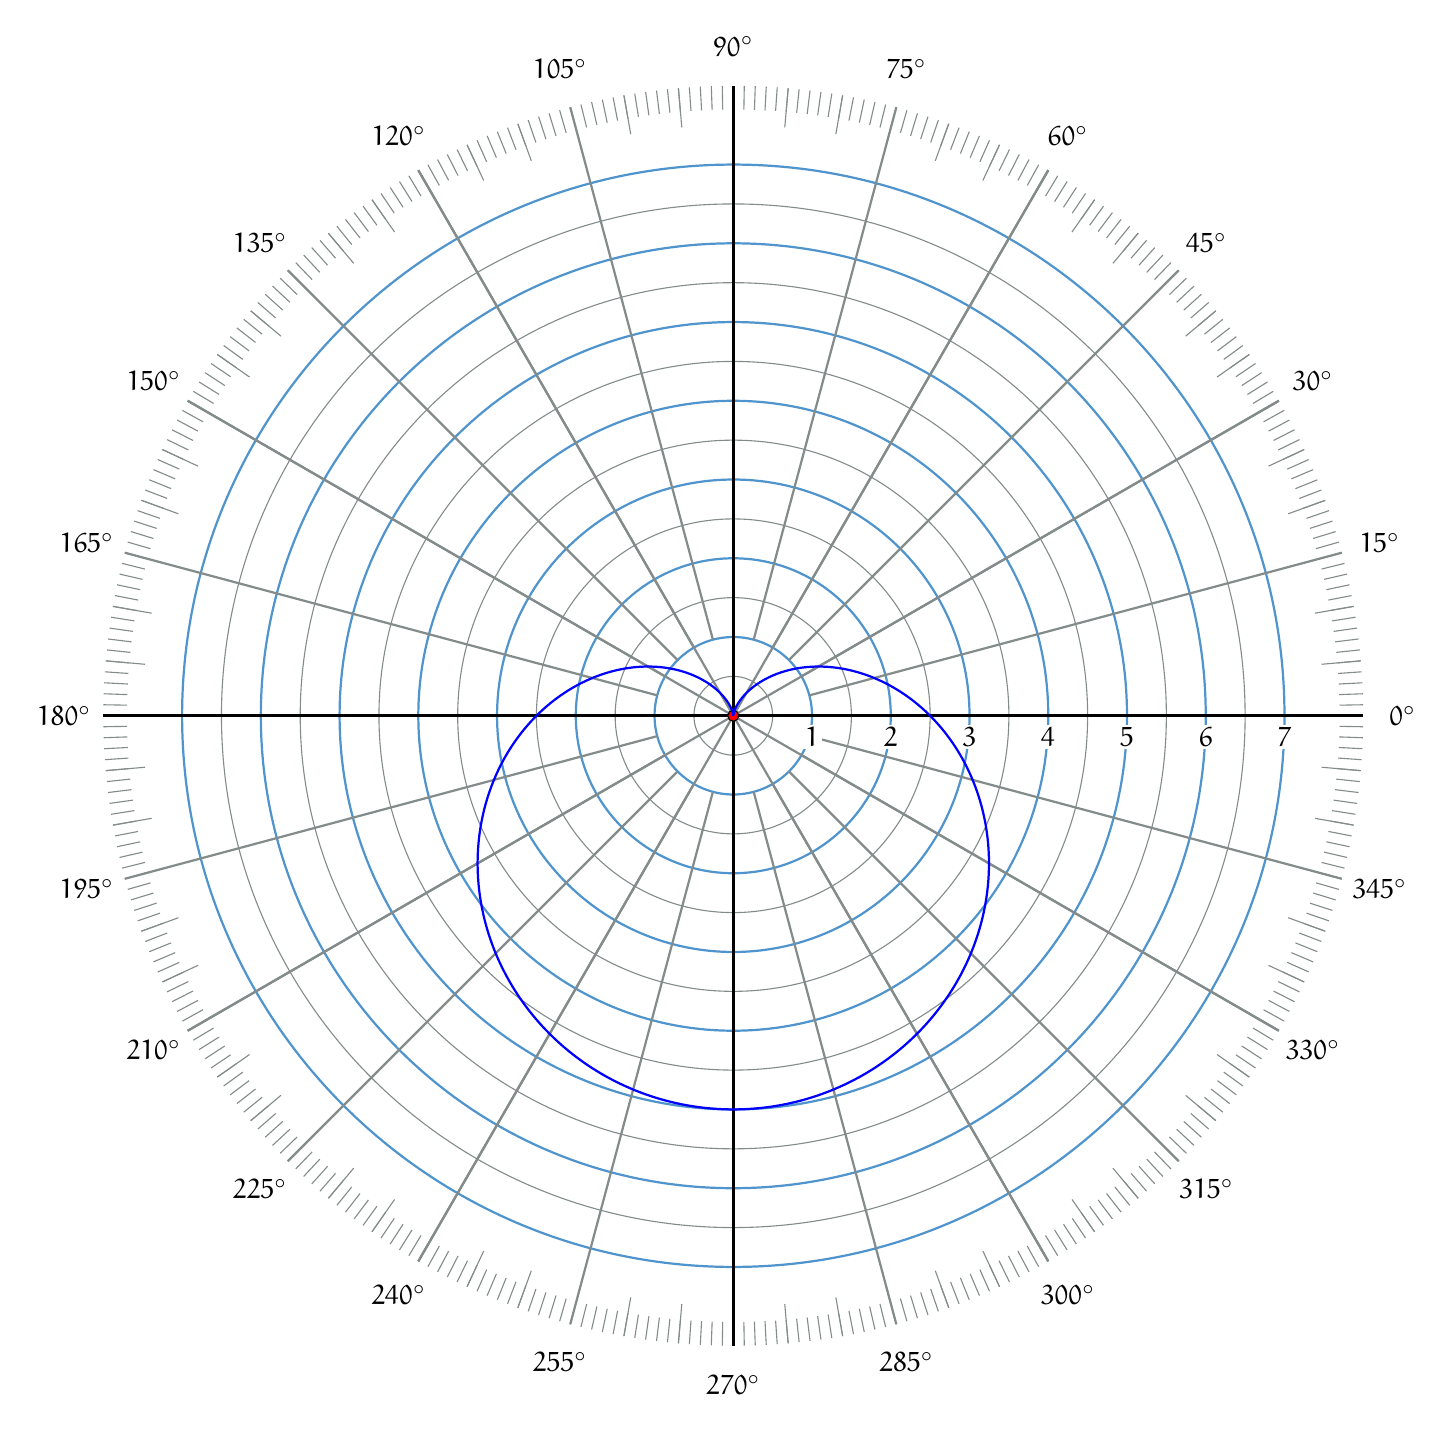
\begin{tikzpicture}
    %Circles 
    \foreach \r in {1, 2,...,7}
    \draw[SteelBlue3, thick] (0,0) circle (\r);    
    \foreach \r in {0.5, 1.5,...,7}
    \draw[Azure4, thin] (0,0) circle (\r);
    %1° Rays
    \foreach \a in {0, 1,...,359}
    \draw[Azure4] (\a:7.7) -- (\a:8);
    %5° Rays
    \foreach \a in {0, 5,...,359}
    \draw[Azure4] (\a:7.5) -- (\a:8);      
    %15° Rays
    \foreach \a in {0, 15,...,359}
    \draw[thick,Azure4] (\a:1) -- (\a:8); 
    %30° Rays
    \foreach \a in {0, 30,...,359}
    \draw[thick,Azure4] (0, 0) -- (\a:8);
    %Radius labels (background filled white)
    \foreach \r in {1, 2,...,7}
    \draw (\r,0) node[inner sep=1pt,below=3pt,rectangle,fill=white] {$\r$};
    %Main rays
    \foreach \a in {0, 90,...,359}
    \draw[very thick] (0, 0) -- (\a:8);
    %Angle labels  
    \foreach \a in {0, 15,...,359}
    \draw (\a: 8.5) node {$\a^\circ$};
    %Central point
    \draw[fill=red] (0,0) circle(0.7mm);
    % Now the additional plot:
    \begin{polaraxis}[hide axis,anchor=origin,disabledatascaling,at={(0pt,0pt)},x=1cm,y=1cm]
    \addplot+[mark=none,domain=0:720,samples=600,thick] 
    {5-5*sin(x)}; 
    \end{polaraxis}
    \end{tikzpicture}
    
%    \begin{tikzpicture}[scale=2]
%    \drawHDYXYaxes
%    \draw node [red] at (-1,.25) {\scriptsize{Kardioida $r=1-\tan
%            \theta$}};
%    \draw[color=red,domain=0:6.28,samples=200,smooth] plot (canvas polar
%    cs:angle=\x r,radius=      {5-5*tan(\x r)});    %r = angle en radian
%    \end{tikzpicture}
%    \resizebox{5cm}{5cm}{
%%        \begin{tikzpicture}[scale=2]
%%        \drawHDYXYaxes
%%        \draw node [red] at (-1,.25) {\scriptsize{Kardioida $r=1+\tan
%%                \theta$}};
%%        \draw[color=red,domain=0:1.5,samples=200,smooth] plot (canvas polar
%%        cs:angle=\x r,radius=      {5+5*tan(\x r)});    %r = angle en radian
%%        \draw[color=red,domain=1.64:3.07,samples=200,smooth] plot (canvas polar
%%        cs:angle=\x r,radius=      {5+5*tan(\x r)});    %r = angle en radian
%%        \draw[color=red,domain=3.21:4.64,samples=200,smooth] plot (canvas polar
%%        cs:angle=\x r,radius=      {5+5*tan(\x r)});    %r = angle en radian
%%        \draw[color=red,domain=4.78:6.28,samples=200,smooth] plot (canvas polar
%%        cs:angle=\x r,radius=      {5+5*tan(\x r)});    %r = angle en radian
%%        \end{tikzpicture}
%    }
\end{document}